% Options for packages loaded elsewhere
\PassOptionsToPackage{unicode}{hyperref}
\PassOptionsToPackage{hyphens}{url}
\PassOptionsToPackage{dvipsnames,svgnames,x11names}{xcolor}
%
\documentclass[
  letterpaper,
  DIV=11,
  numbers=noendperiod]{scrartcl}

\usepackage{amsmath,amssymb}
\usepackage{iftex}
\ifPDFTeX
  \usepackage[T1]{fontenc}
  \usepackage[utf8]{inputenc}
  \usepackage{textcomp} % provide euro and other symbols
\else % if luatex or xetex
  \usepackage{unicode-math}
  \defaultfontfeatures{Scale=MatchLowercase}
  \defaultfontfeatures[\rmfamily]{Ligatures=TeX,Scale=1}
\fi
\usepackage{lmodern}
\ifPDFTeX\else  
    % xetex/luatex font selection
\fi
% Use upquote if available, for straight quotes in verbatim environments
\IfFileExists{upquote.sty}{\usepackage{upquote}}{}
\IfFileExists{microtype.sty}{% use microtype if available
  \usepackage[]{microtype}
  \UseMicrotypeSet[protrusion]{basicmath} % disable protrusion for tt fonts
}{}
\makeatletter
\@ifundefined{KOMAClassName}{% if non-KOMA class
  \IfFileExists{parskip.sty}{%
    \usepackage{parskip}
  }{% else
    \setlength{\parindent}{0pt}
    \setlength{\parskip}{6pt plus 2pt minus 1pt}}
}{% if KOMA class
  \KOMAoptions{parskip=half}}
\makeatother
\usepackage{xcolor}
\setlength{\emergencystretch}{3em} % prevent overfull lines
\setcounter{secnumdepth}{-\maxdimen} % remove section numbering
% Make \paragraph and \subparagraph free-standing
\ifx\paragraph\undefined\else
  \let\oldparagraph\paragraph
  \renewcommand{\paragraph}[1]{\oldparagraph{#1}\mbox{}}
\fi
\ifx\subparagraph\undefined\else
  \let\oldsubparagraph\subparagraph
  \renewcommand{\subparagraph}[1]{\oldsubparagraph{#1}\mbox{}}
\fi


\providecommand{\tightlist}{%
  \setlength{\itemsep}{0pt}\setlength{\parskip}{0pt}}\usepackage{longtable,booktabs,array}
\usepackage{calc} % for calculating minipage widths
% Correct order of tables after \paragraph or \subparagraph
\usepackage{etoolbox}
\makeatletter
\patchcmd\longtable{\par}{\if@noskipsec\mbox{}\fi\par}{}{}
\makeatother
% Allow footnotes in longtable head/foot
\IfFileExists{footnotehyper.sty}{\usepackage{footnotehyper}}{\usepackage{footnote}}
\makesavenoteenv{longtable}
\usepackage{graphicx}
\makeatletter
\def\maxwidth{\ifdim\Gin@nat@width>\linewidth\linewidth\else\Gin@nat@width\fi}
\def\maxheight{\ifdim\Gin@nat@height>\textheight\textheight\else\Gin@nat@height\fi}
\makeatother
% Scale images if necessary, so that they will not overflow the page
% margins by default, and it is still possible to overwrite the defaults
% using explicit options in \includegraphics[width, height, ...]{}
\setkeys{Gin}{width=\maxwidth,height=\maxheight,keepaspectratio}
% Set default figure placement to htbp
\makeatletter
\def\fps@figure{htbp}
\makeatother
\newlength{\cslhangindent}
\setlength{\cslhangindent}{1.5em}
\newlength{\csllabelwidth}
\setlength{\csllabelwidth}{3em}
\newlength{\cslentryspacingunit} % times entry-spacing
\setlength{\cslentryspacingunit}{\parskip}
\newenvironment{CSLReferences}[2] % #1 hanging-ident, #2 entry spacing
 {% don't indent paragraphs
  \setlength{\parindent}{0pt}
  % turn on hanging indent if param 1 is 1
  \ifodd #1
  \let\oldpar\par
  \def\par{\hangindent=\cslhangindent\oldpar}
  \fi
  % set entry spacing
  \setlength{\parskip}{#2\cslentryspacingunit}
 }%
 {}
\usepackage{calc}
\newcommand{\CSLBlock}[1]{#1\hfill\break}
\newcommand{\CSLLeftMargin}[1]{\parbox[t]{\csllabelwidth}{#1}}
\newcommand{\CSLRightInline}[1]{\parbox[t]{\linewidth - \csllabelwidth}{#1}\break}
\newcommand{\CSLIndent}[1]{\hspace{\cslhangindent}#1}

\KOMAoption{captions}{tableheading}
\makeatletter
\makeatother
\makeatletter
\makeatother
\makeatletter
\@ifpackageloaded{caption}{}{\usepackage{caption}}
\AtBeginDocument{%
\ifdefined\contentsname
  \renewcommand*\contentsname{Table of contents}
\else
  \newcommand\contentsname{Table of contents}
\fi
\ifdefined\listfigurename
  \renewcommand*\listfigurename{List of Figures}
\else
  \newcommand\listfigurename{List of Figures}
\fi
\ifdefined\listtablename
  \renewcommand*\listtablename{List of Tables}
\else
  \newcommand\listtablename{List of Tables}
\fi
\ifdefined\figurename
  \renewcommand*\figurename{Figure}
\else
  \newcommand\figurename{Figure}
\fi
\ifdefined\tablename
  \renewcommand*\tablename{Table}
\else
  \newcommand\tablename{Table}
\fi
}
\@ifpackageloaded{float}{}{\usepackage{float}}
\floatstyle{ruled}
\@ifundefined{c@chapter}{\newfloat{codelisting}{h}{lop}}{\newfloat{codelisting}{h}{lop}[chapter]}
\floatname{codelisting}{Listing}
\newcommand*\listoflistings{\listof{codelisting}{List of Listings}}
\makeatother
\makeatletter
\@ifpackageloaded{caption}{}{\usepackage{caption}}
\@ifpackageloaded{subcaption}{}{\usepackage{subcaption}}
\makeatother
\makeatletter
\@ifpackageloaded{tcolorbox}{}{\usepackage[skins,breakable]{tcolorbox}}
\makeatother
\makeatletter
\@ifundefined{shadecolor}{\definecolor{shadecolor}{rgb}{.97, .97, .97}}
\makeatother
\makeatletter
\makeatother
\makeatletter
\makeatother
\ifLuaTeX
  \usepackage{selnolig}  % disable illegal ligatures
\fi
\IfFileExists{bookmark.sty}{\usepackage{bookmark}}{\usepackage{hyperref}}
\IfFileExists{xurl.sty}{\usepackage{xurl}}{} % add URL line breaks if available
\urlstyle{same} % disable monospaced font for URLs
\hypersetup{
  pdftitle={The Effects of Fiscal Policy Shifts on Unemployment Rates},
  pdfauthor={Yansong Yang},
  colorlinks=true,
  linkcolor={blue},
  filecolor={Maroon},
  citecolor={Blue},
  urlcolor={Blue},
  pdfcreator={LaTeX via pandoc}}

\title{The Effects of Fiscal Policy Shifts on Unemployment Rates}
\author{Yansong Yang}
\date{}

\begin{document}
\maketitle
\ifdefined\Shaded\renewenvironment{Shaded}{\begin{tcolorbox}[sharp corners, interior hidden, breakable, frame hidden, boxrule=0pt, enhanced, borderline west={3pt}{0pt}{shadecolor}]}{\end{tcolorbox}}\fi

\begin{quote}
\textbf{Abstract.} This study investigates the dynamic impact of fiscal
policy shifts on unemployment rates through a Structural Vector
Autoregression (SVAR) model. Utilizing time series data for government
spending, tax revenue, inflation, and unemployment rates, we analyze the
interplay between fiscal activities and labor market performance within
an Australian context. The SVAR model, equipped to dissect the influence
of systematic fiscal shocks, reveals insights into how fiscal policy
affects employment.

\textbf{Keywords.} svars, fiscal policy, unemployment rates, government
spending, tax revenue, inflation
\end{quote}

\hypertarget{the-question-objective-and-motivation}{%
\section{1. The Question, Objective, and
Motivation}\label{the-question-objective-and-motivation}}

The objective of this research project is to assess the effects of
fiscal policy shifts on unemployment rates. I aim to investigate how
unemployment rates respond to changes in government spending and
taxation under various fiscal policy frameworks.

Unemployment is pivotal in the macroeconomic framework, directly tied to
social welfare and economic performance. Considering the economic
challenges faced by Australia, the examination of fiscal policy's
influence on unemployment is timely. For instance, Leigh (2012) found
that fiscal consolidation efforts in Australia could potentially lift
unemployment rates in the short term. Chapman and Kapuscinski (2000)
identified that the Australian labor market exhibits notable sensitivity
to macroeconomic policy shifts, with fiscal measures playing a
significant role in shaping employment trends. These findings have
piqued my curiosity about understanding fiscal policy mechanisms in the
Australian labor market. By conducting this research, I aim to provide
an updated empirical analysis of how contemporary fiscal policy
adjustments are impacting unemployment rates in Australia, thereby
offering insights that may inform policy refinement for enhanced
economic resilience and labor stability.

\hypertarget{data-and-their-properties}{%
\section{2. Data and Their Properties}\label{data-and-their-properties}}

\hypertarget{variables-selected}{%
\subsection{2.1 Variables Selected}\label{variables-selected}}

Unemployment Rate (UNEMP): Monthly data on the unemployment rate in
Australia, sourced from the Australian Bureau of Statistics (ABS). In
further steps, it will be converted to quarterly data.

Government Spending (GOVSPEND): Quarterly data on total government
expenditure, including both consumption and investment, also obtained
from ABS.

Tax Revenue (TAXREV): Quarterly tax revenue data for the Australian
government, which can be sourced from ABS.

Inflation Rate (INFL): The consumer price index (CPI) from which the
quarterly inflation rate can be calculated, available from ABS.

Real Gross Domestic Product (RGDP): Quarterly data of the value of all
goods and services produced by Australia, adjusted for inflation.
Sourced from RBA.

Cash Rate Target(CR): Quarterly data of the interest rate that banks pay
to borrow funds from central banks in the overnight markets, set by RBA.

\hypertarget{why-chose-them}{%
\subsection{2.2 Why Chose Them?}\label{why-chose-them}}

The chosen variables are integral to capturing the broad dynamics of
fiscal policy and its impact on the labor market. The unemployment rate
(UNEMP) is the direct indicator of labor market health. Government
spending (GOVSPEND) and tax revenue (TAXREV) are key fiscal policy tools
that directly affect aggregate demand, and by extension, employment and
output. Inflation rate (INFL) is a crucial economic indicator that can
reflect the demand-pull effects in the economy which, in a Keynesian
context, may affect the level of employment. Real GDP(RGDP) is included
as it reflects the overall economic output and health, directly
correlating with job market strength. The cash rate(CR) is a measure of
monetary policy influence on fiscal effectiveness and employment levels.

\hypertarget{data-visualization}{%
\subsection{2.3 Data Visualization}\label{data-visualization}}

The time series plots{[}Figure 1: Time Series Data{]} for unemployment
rate, government spending, tax revenue, and inflation collectively offer
a glimpse into the interplay between fiscal policy and economic
indicators in an economy. The unemployment rate displays cyclical
patterns with notable spikes, hinting at its sensitivity to economic
conditions and potentially reactive fiscal policies. The upward
trajectories of both government spending and tax revenue suggest an
expanding fiscal capacity over time, likely driven by both economic
growth and policy decisions.

Government spending's steady rise, with occasional steeper inclines,
could imply proactive fiscal stimulus during periods of economic
downturn, which often sees a lagged corresponding dip in the
unemployment rate. Tax revenue's increase, while generally consistent
with economic growth, also shows sensitivity to business cycles,
indicating that it's both a reflection of and a contributor to the
fiscal environment. Inflation's volatility is without a clear trend
line.

These time series hint at a complex relationship where fiscal policy,
through government spending and tax revenue, aims to moderate the
impacts of economic cycles on unemployment, all while operating within
the broader context influenced by inflation dynamics. The ebb and flow
in these indicators reflect the challenges and responses in managing an
economy over time.

\begin{figure}

\begin{minipage}[t]{\linewidth}

{\centering 

\raisebox{-\height}{

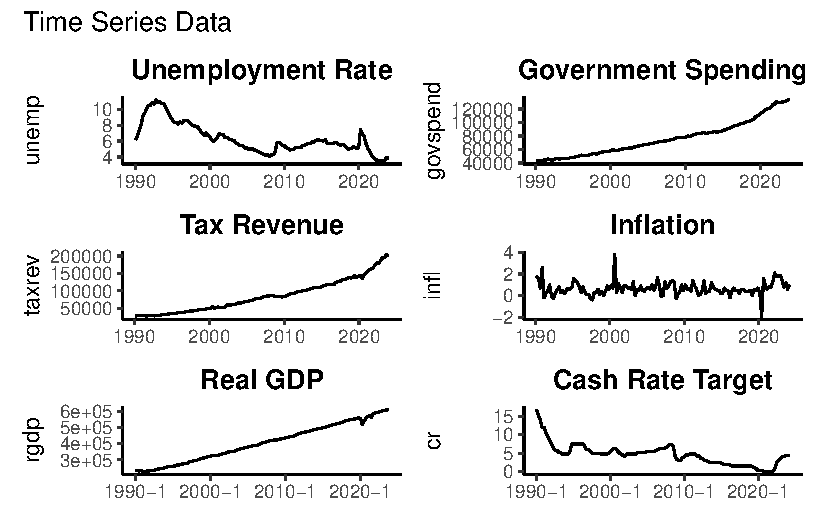
\includegraphics{index_files/figure-pdf/unnamed-chunk-2-1.pdf}

}

\caption{Time Series Data}

}

\end{minipage}%

\end{figure}

\hypertarget{property-tested}{%
\subsection{2.4 Property Tested}\label{property-tested}}

From the ACF test{[}Figure 2: Autocorrelation Function{]}, the
unemployment rate shows a strong initial correlation that quickly tails
off, indicating that past unemployment only affects the current rate for
a short period. Government spending and tax revenue, on the other hand,
display more prolonged correlations, suggesting that current values are
influenced by a longer history of the series. This persistence might be
a sign of a trend or other non-stationary behavior in the series.
Inflation shows some initial correlation that diminishes, which could be
indicative of cyclical behavior being smoothed out over time.

From the PACF test{[}Figure 3: Partial Autocorrelation Function{]}, for
unemployment, there's a significant direct correlation with the
immediate past, which is not seen in the following lags. This indicates
that other than the most recent past, there's little direct effect on
the current unemployment rate. In the case of government spending, tax
revenue, and inflation, the PACF plots suggest that after accounting for
other factors, the direct correlations are quite minimal. This could
imply that these time series are driven by a more complex set of factors
than just their immediate past values.

\begin{figure}

{\centering 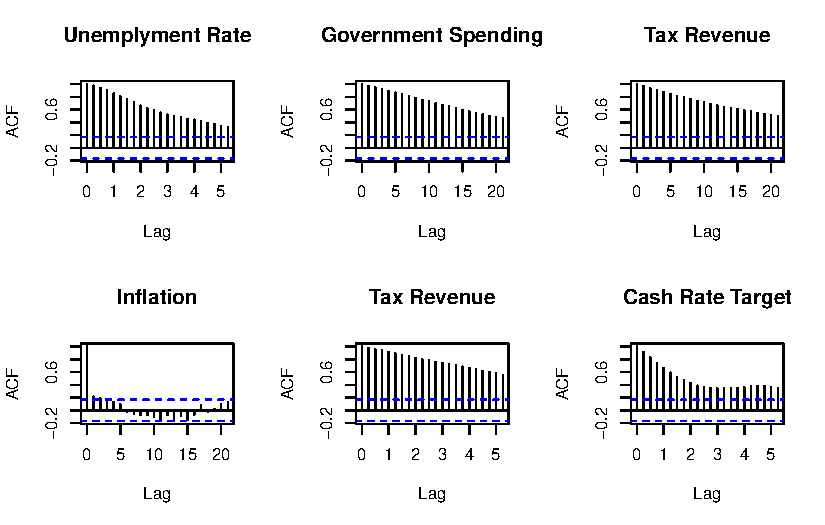
\includegraphics[width=0.8\textwidth,height=\textheight]{index_files/figure-pdf/unnamed-chunk-3-1.pdf}

}

\caption{Autocorrelation Function}

\end{figure}

\begin{figure}

{\centering 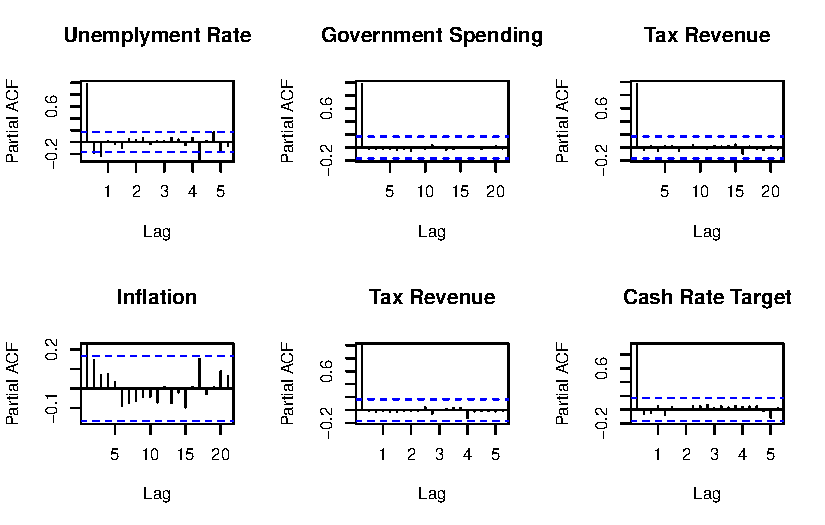
\includegraphics[width=0.8\textwidth,height=\textheight]{index_files/figure-pdf/unnamed-chunk-4-1.pdf}

}

\caption{Partial Autocorrelation Function}

\end{figure}

\hypertarget{the-model-and-hypothesis}{%
\section{3. The Model and Hypothesis}\label{the-model-and-hypothesis}}

\hypertarget{model}{%
\subsection{3.1 Model}\label{model}}

The \textbf{Structural Form (SF) model} of Structural VARs is:

\[
\begin{align}
B_{0} Y_{t} =b_{0}  + \sum_{i=0}^{p} (B_{i}Y_{t-i} )+u_{t} 
\end{align}
\] \[
\begin{align}
u_{t}|Y_{t-1} \sim iid(0_{N},I_{N}  )
\end{align}
\] - \(Y_{t}\) is \(N \times 1\) matrix of endogenous variable.

\begin{itemize}
\item
  \(B_{0}\) is \(N \times N\) matrix of contemporaneous relationships
  also called structural matrix. It captures contemporaneous
  relationships between variables.
\item
  \(u_{t}\) is a \(N \times 1\) vector of conditionally
  on\(Y_{t-1}\)orthogonal or independent structural shocks. Isolating
  these shocks allows us to identify dynamic effects of uncorrelated
  shocks on variables \(Y_{t}\).
\end{itemize}

The \textbf{Reduced Form (RF)} representation is:

\[
\begin{align}
Y_{t} =\mu_{0}  + \sum_{i=0}^{p} (A_{i}Y_{t-i} )+\epsilon_{t} 
\end{align}
\]

\[
\begin{align}
\epsilon_{t}|Y_{t-1} \sim iid(0_{N},\Sigma )
\end{align}
\] Either of the SF models lead to the same RF representation through
various equivalence transformations

\[
\epsilon_t = B u_t = B_0^{-1} u_t
\]

\[
B_0 \epsilon_t = u_t
\]

\[
\Sigma = BB' = B_0^{-1} B_0'^{-1}
\]

\hypertarget{deriviation}{%
\subsection{3.2 Deriviation}\label{deriviation}}

The first step is to sample the reduced-form parameters (\(\*A\),
\(\*\Sigma\)). Adopting the conjugate Normal-Inverse-Wishart prior,

\[
\begin{align*}
\mathbf{A}|\mathbf{\Sigma} &\sim \mathcal{MN}_{K \times N}(\underline{\mathbf{A}}, \underline{\mathbf{V}}, \mathbf{\Sigma}) \\
\mathbf{\Sigma} &\sim \mathcal{IW}_N(\underline{\mathbf{S}}, \underline{\nu})
\end{align*}
\]

and let

\[
\begin{align*}
\hat{A} &= (X'X)^{-1}X'Y \\
R &= (Y - X\hat{A})'(Y - X\hat{A})
\end{align*}
\]

\hypertarget{hypothesis}{%
\subsection{3.3 Hypothesis}\label{hypothesis}}

Here are the hypotheses I am interested in:

\begin{enumerate}
\def\labelenumi{\arabic{enumi}.}
\item
  Counter-Cyclical Government Spending Hypothesis: Increases in
  government spending during periods of rising unemployment act as a
  counter-cyclical tool to stimulate economic activity and lower
  unemployment rates.
\item
  Tax Revenue and Economic Activity Hypothesis: An increase in tax
  revenue due to economic growth might coincide with lower unemployment
  rates, an increase due solely to higher tax rates might suppress
  economic activity and potentially increase unemployment.
\item
  Fiscal Policy Impact Lag Hypothesis: Given that fiscal policy changes
  do not have an immediate effect, we hypothesize that there are lags in
  the impact of government spending and tax changes on the unemployment
  rate.
\end{enumerate}

\hypertarget{references}{%
\subsection*{References}\label{references}}
\addcontentsline{toc}{subsection}{References}

\hypertarget{refs}{}
\begin{CSLReferences}{1}{0}
\leavevmode\vadjust pre{\hypertarget{ref-Chapman2000AvoidingRA}{}}%
Chapman, Bruce, and Cezary A. Kapuscinski. 2000. {``Avoiding Recessions
and Australian Long-Term Unemployment.''} In.
\url{https://api.semanticscholar.org/CorpusID:152681286}.

\leavevmode\vadjust pre{\hypertarget{ref-leigh2012}{}}%
Leigh, Andrew. 2012. {``How Much Did the 2009 Australian Fiscal Stimulus
Boost Demand? Evidence from Household-Reported Spending Effects.''}
\emph{The B.E. Journal of Macroeconomics} 12 (1).
\url{https://doi.org/10.1515/1935-1690.2035}.

\end{CSLReferences}



\end{document}
